\documentclass{standalone}

\usepackage{circuitikz}

\begin{document}

% INT_AY21_L29_Fig09_Field_at_point.png

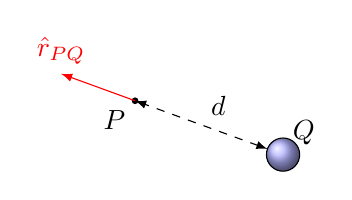
\begin{tikzpicture}[> = latex]

	% Charge Q
	
	\draw [ball color = blue!30] (0, 0) circle (6 pt) node [above right] {$Q$};
	
	% Point P w/ unit vector
	
	\filldraw (160 : 2) circle (1 pt) node [below left] {$P$};
	\draw [red, ->] (160 : 2) -- ++ (160 : 1) node [above] {${\hat r}_{PQ}$};
	
	% Distance indicator
	
	\draw [dashed, <->] (160 : 6 pt) -- node [above right] {$d$} (160 : 2);
	
\end{tikzpicture}

\end{document}